\section{Serverless Computing}
% got 4 pages
This section aims to give an overview of serverless computing.
Readers who are well-versed within the matter can feel free to skip this introduction, and reference it only when needed
\subsection{What serverless computing is}
Serverless computing emerged as a new computing paradigm in the context of cloud computing, which delegates infrastructure provisioning and configuration to the cloud provider to alleviate software developers from that burden.
\gls{faas} is one of the most prominent types of serverless computing products on offer.
It allows developers to specify serverless functions, which are then deployed and scaled by the cloud provider.
It is a way in which software developers architect, develop, and deploy applications that is dramatically different from more traditional approaches.
In traditional approaches, such as microservice architectures, an application is partitioned into small components which can be scaled and deployed independently of each other.
Although microservice architectures often rely on the \gls{iaas} or \gls{paas} solutions cloud providers offer, and thus abstract away the underlying infrastructure to a certain degree, developers still need to handle most scaling and application specific \gls{qos} requirements themselves.

From a developer's perspective, serverless computing is a further increase in abstraction \cite{jonasCloudProgrammingSimplified2019}.
It can be seen as the next step in an evolution away from monolithic software applications.
Where microservices and containerized deployments first partitioned a large application into several smaller applications, serverless computing continues this trend of division into smaller components, since in serverless computing applications are partitioned into individual \textit{functions}, which each perform a single action\cite{khandelwalTaureauDeconstructingServerless2020}.

\begin{figure}
    \centering
    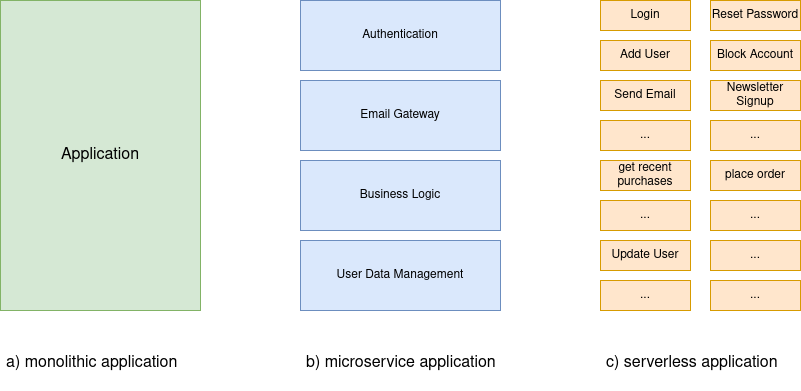
\includegraphics[width=\columnwidth]{graphics/diagrams/monolith_micro_serverless.png}
    \caption{Conceptual overview of different application architecture paradigms}
    \label{fig:mono_micro_serverless}
\end{figure}

Figure \ref{fig:mono_micro_serverless} shows this transition towards smaller partitioning of application code, leading to a higher and higher level of abstraction.
Just like microservices enabled application developers to scale different aspects of an application independently, thus enabling elasticity, serverless computing takes this even further allowing individual functions of the application to be scaled separately from each other\cite{jonasCloudProgrammingSimplified2019}.

Overall serverless affords application developers a number of advantages:
\begin{itemize}
    \item \textbf{Arbitrary elasticity:} As mentioned, serverless applications can scale their components on an extremely fine-grained level\cite{khandelwalTaureauDeconstructingServerless2020}
    \item \textbf{Abstracted infrastructure:} Where previously developers needed to be at least somewhat cognizant of the deployment of their application or its microservices, serverless enables this task to be fully delegated to the cloud provider. Developers don't necessarily need any knowledge of cloud infrastructure\cite{jonasCloudProgrammingSimplified2019}.
    \item \textbf{Precise Billing:} While in traditional cloud computing environments resources are leased for a set amount of time, irrespective of their actual usage\cite{khandelwalTaureauDeconstructingServerless2020}, serverless features a billing model where only the actual execution time and memory footprint of a function is billed down to millisecond precision\cite{jonasCloudProgrammingSimplified2019}. This allows for better resource utilization and potentially reduced costs from a customer's perspective\cite{khandelwalTaureauDeconstructingServerless2020}.
\end{itemize}

While these advantages of serverless computing over more traditional approaches are compelling, there are also idiosyncrasies of serverless computing that can, depending on the application, be problematic.
These include the need for statelessness, meaning that serverless functions have no inherent capacity to store data and would instead need to fetch it from yet another service\cite{khandelwalTaureauDeconstructingServerless2020}, or potential performance inconsistencies from cold-starts.
A cold-start, which means that the specific function code isn't running and has to be started before the request can be serviced, can occur because a serverless function wasn't executed for a certain time\cite{wangPeekingCurtainsServerless2018}.

\subsection{The architecture of serverless systems}
Architecturally, serverless systems are closely related to event based systems.
Their general concept is also very similar, since an event (i.e. a request) first arrives at the system in a form of queue, where a dispatcher or load balancer decides what action needs to be taken based on the event, and forwards it to the service (i.e. function), which ultimately processes it\cite{castroServerDeadLong2019}.

Prominent cloud based serverless platforms such as AWS Lambda\cite{aws-lambda} and Azure Functions\cite{azure-functions} are, however, proprietary and their precise architecture and inner workings are thus unknown to the public.
How these systems behave is a topic of ongoing research\cite{wangPeekingCurtainsServerless2018}, but since our research requires precise knowledge of implementation details, we choose to use open source serverless frameworks as a reference architecture of serverless systems.
These systems include Apache OpenWhisk\cite{openwhisk}, Kubeless\cite{kubeless}, and OpenFaaS\cite{openfaas}.
Since OpenFaaS has already been adapted for serverless edge computing by Rausch et al.\cite{rauschServerlessPlatformEdge}, we choose to use this open source serverless framework as the stand-in for serverless computing frameworks in general.

Architecturally, OpenFaaS is structured very similarly to the generic serverless architecture described by Castro et al.\cite{castroServerDeadLong2019}.
It too has a centralized entry-point, the Gateway, which sends requests to specific function replicas or alternatively to a queue (used for asynchronous processing and dealing with requests to functions that aren't currently running).
Each Gateway is thus effectively a load balancer for the serverless functions.
Figure \ref{fig:openfaas-gateway-diagram} shows a diagram of the architecture, as it is found in their official documentation\cite{openfaas-gateway}.

From a technical perspective, a key aspect of OpenFaaS' implementation is that it uses containers to host functions.
Containers provide an abstraction over Linux based operating systems, allowing for easier management of software dependencies, more closely controlled execution environments, and stronger application isolation.
Each function is packaged into such a container, which is an almost fully self-contained and portable artifact, that allows executing the developers' code on any machine with a compatible container runtime.
Functionally they behave similar to virtual machines, although they start up much faster, and aren't actually running individual kernels, which is why they do not provide the same level of security isolation true virtual machines do.
This choice allows functions to execute reliably, no matter the environment, and also makes it entirely agnostic to the programming language developers wish to use.
Since using containers entails their management over a cluster of multiple nodes, a task which is extremely complex, OpenFaaS\cite{openfaas} as well as other serverless frameworks build on Kubernetes\cite{kubernetes}, the de-facto industry standard container orchestration and management platform.
Building upon Kubernetes to deal with container management is a common choice among open source serverless frameworks, a choice which OpenWhisk and Kubeless make as well\cite{mohantyEvaluationOpenSource2018}.

OpenFaaS delegates a large number of tasks to the underlying Kubernetes cluster, including name resolution, request routing, which includes load balancing, and potentially scaling.
For this work, the delegation of load balancing decisions is especially important, since it implies that OpenFaaS uses whichever load balancing algorithm Kubernetes uses internally to distribute requests among function replicas.
Scaling, which determines how many instances of a serverless functions are running at any given time, can work via different mechanisms in OpenFaaS.
Depending how OpenFaaS is configured, it can either use Kubernetes' integrated \gls{hpa}\cite{kubernetes-hpa} or its own internal mechanism, which optionally allows for user customized scaling behavior\cite{openfaas-autoscaling}.
Since this work also aims to explore the impact a change in scaling and scheduling load balancers can have on the behavior of these scaling systems in general, we will now briefly describe the default scaling behavior of both \gls{hpa} and OpenFaaS' own scaler.

\subsubsection{Kubernets \gls{hpa}}
In Kubernetes scaling is typically based on either CPU or memory utilization, although in principle it can be extended with user-provided custom metrics\cite{kubernetes-hpa}.
For a given deployment, which in the context of serverless computing would be a function, a target resource value is defined.
An example would be a target average CPU utilization of 50\% for a type of function.
At that point, Kubernetes decides in a linear fashion what the desired number of replicas is.

Let $\mathbf{r_{\text{current}}}$ be the number of current replicas, $\mathbf{m_{\text{current}}}$ the current value of the metric in question and $\mathbf{m_{\text{target}}}$ the target value of the metric.
Then the target replica count is

\[ r_{\text{target}} = \left \lceil r_{\text{current}} \times \frac{m_{\text{current}}}{m_{\text{target}}} \right \rceil\]

To prevent inconsistent behavior such as replica counts oscillating Kubernetes also allows certain limiters to be set, such as minimum and maximum scales, rate of change for adding or removing replicas, and cool-downs which give the system time to stabilize before new scaling decisions are considered\cite{kubernetes-hpa}.

\subsubsection{OpenFaaS scaling}
The OpenFaaS integrated scaling mechanism is comprised of different parameters.
First a minimum and maximum scale must be set, which determine the effect of the scaling factor.
In this custom scaling variant system parameters, such as the request rate of a given function, are continuously evaluated.
Once a configured condition is met the system is notified that a given function needs to scale up or down.
The aforementioned scaling factor, which is a percentage value between 0 and 100, is then used to determine how many replicas should be started or stopped\cite{openfaas-autoscaling}.
Each scaling iteration adds or removes a number of replicas relative to the maximum scale allowed, and the scaling factor determines the size of that share.
If, for example, the maximum number of replicas is 50, and the scaling factor is 10\%, then at each scaling operation 5 replicas will be added or removed.

Which exact conditions trigger a scale up or scale down event within OpenFaaS is extremely configurable, and allows for customization based on an individual function's requirements.
By default, OpenFaaS triggers a scale-up event if the rate of rise of a function's invocation frequency exceeds a threshold over a period of time.



